 
\chapter{Dados Obtidos}
\label{cap6}
%ccm Não esquecer de zerar o eixo X
%ccm todo gráfico precisa responder a alguma pergunta.
% 1- Formular a pergunta com base no que definiu no Cap.4
% 2- quem está envolvido, quais são os parâmetros, quais são constantes
% 3- Descrever o perfil/modus operandi do experimento
% 4- Mostra a figura
% 5- Analisa os resultados com base na expectativa no Cap.4 (foi similar, diferente, por quê?)
% 6 - Precisa manter em mente que as figuras devem manter uma escala para poder comparar entre diferentes arquiteturas

\section{Dados obtidos da arquitetura Rudy}

Para obter os dados da arquitetura Rudy, foram efetuadas 3 testes diferentes.
%
Em específico, a diferença entre cada teste é o crescimento de conexões por minuto.
%
Os testes foram automatizados da seguinte maneira:

\begin{itemize}
 \item Utilizando uma conta nova por minuto.
 \item Utilizando duas contas novas por minuto.
 \item Utilizando cinco contas novas por minuto.
\end{itemize}

Para cada ítem citado, a cada minuto, é escalonado um novo cliente robô que realizará as seguintes ações:

\begin{itemize}
 \item Criar uma conta.
 \item Autenticar a conta.
 \item Criar um personagem.
 \item Selecionar personagem.
 \item Movimentar-se pelo jogo, enviar mensagens e receber mensagens.
\end{itemize}

Dentro deste cenário, espera-se estressar a vazão da rede ou \ac{cpu}, visto que são poucos dados para armazenamento em memória do serviço de jogo.
%
Vale ressaltar que a latência da rede não foi prejudicada durante o teste, tornando-se constante, como já esperado.


\section{Consumo de CPU na arquitetura Rudy}

Um dos objetivos da coleta de \ac{cpu} da arquitetura Rudy é analisar pontos de gargalo.
%
Em especial a arquitetura Rudy tem uma abordagem serial das requisições, a qual serve para evitar a concorrência das estruturas de dados entre múltiplos jogadores.

Esta abordagem é comum para jogos onde a frequência de atualizações é menor, visto que seu principal fator limitante é a fila de requisições.
%
Dessa forma, espera-se obter um teto limite de \ac{cpu} durante a análise.

As variáveis relacionadas a este teste são o número de conexões.
%
Na Figura~\ref{fig:rudy_t4_cpu} exibe a carga da \ac{cpu}.


\begin{figure}[htb!]
    \ref{fig:rudy_t4_cpu}
    \caption{Tempo de requisição a partir dos Clientes}
    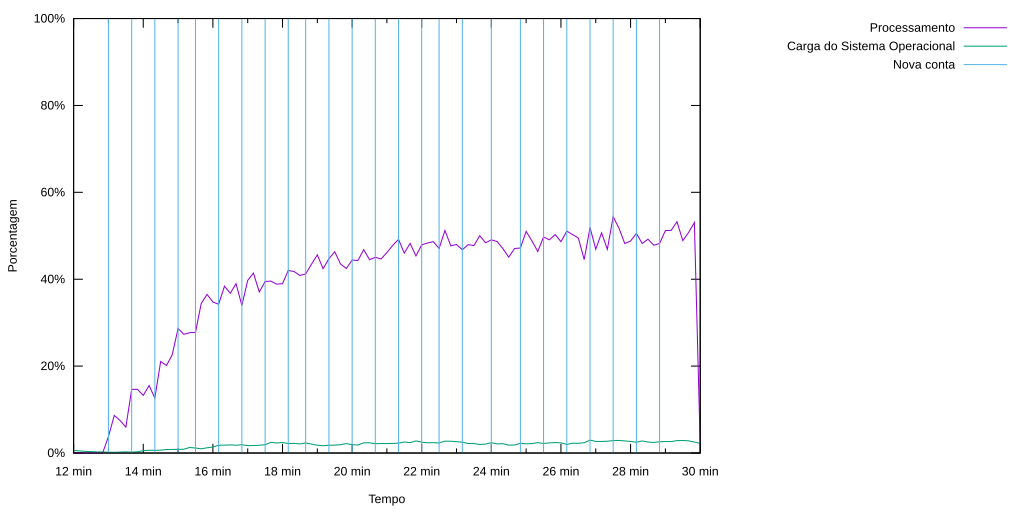
\includegraphics[width=\textwidth]{metricas_rudy_t4/cpu.png}
    \centering
    
    Fonte: O próprio autor
\end{figure}

